\documentclass[conference]{IEEEtran}
\IEEEoverridecommandlockouts
% The preceding line is only needed to identify funding in the first footnote. If that is unneeded, please comment it out.
\usepackage{cite}
\usepackage{amsmath,amssymb,amsfonts}
\usepackage{algorithmic}
\usepackage{graphicx}
\usepackage{textcomp}
\usepackage{xcolor}
\def\BibTeX{{\rm B\kern-.05em{\sc i\kern-.025em b}\kern-.08em
    T\kern-.1667em\lower.7ex\hbox{E}\kern-.125emX}}
\begin{document}

\title{Real-time Domain Adaptation in Semantic Segmentation*\\
{\footnotesize \textsuperscript{*}Note: Sub-titles are not captured in Xplore and
should not be used}
}

\author{\IEEEauthorblockN{1\textsuperscript{st} Berardo Nicholas}
\IEEEauthorblockA{\textit{dept. Computer Engineering} \\
\textit{Politecnico di Torino}\\
Turin, Italy \\
s319349@studenti.polito.it}
\and
\IEEEauthorblockN{2\textsuperscript{nd} Cardona Riccardo}
\IEEEauthorblockA{\textit{dept. Computer Engineering} \\
\textit{Politecnico di Torino}\\
Turin, Italy \\
s319441@studenti.polito.it}
\and
\IEEEauthorblockN{3\textsuperscript{rd} De Marco Alessando}
\IEEEauthorblockA{\textit{dept. Computer Engineering} \\
\textit{Politecnico di Torino}\\
Turin, Italy \\
sXXXXXX@studenti.polito.it}
}

\maketitle

\begin{abstract}
We use an efficient structure named Short-Term Dense Concatenate network (STDC network) for the semantic segmentation task. This
structre reduce the dimension of feature maps and use the aggregation of them for image representation, then use a Detail aggregation
module for producing the low-level features. Finally these two are merged to produce the segmentation result. We test this model on 
Cityscapes and GTA V, following the evaluation of the domain shift between GTA V and Cityscapes and finally we implement and 
unsupervised adversarial domain adaptation method used for reducing the domain shift. We also show the result for the STDC network in
term of mIoU and the result for the domain adaptation. 
\end{abstract}


\section{Introduction}
Semantic Segmentation is a topic in computer vision that aims at assigning a label to each pixel of the image. This is used in many fields
such as autonomous veichle, video surveillance and robot sensing. There are a lot of models that can achive good accuracy. For real-time
semantic segmentation some models choose lightweight backbones for having an increase of performance but a drastic drop of accuracy. For
this reason some new methods were investigated, like feature fusion or aggregation modules. Other models reduce the input image size 
but this can result in a bad accuracy around boundaries and small object. 

STDC net \cite{b1} uses the first approach. Fig.~\ref{stdc_net} shows how the image is encoded in different scales. The kernel size is also reduced
to speed-up the performance but with an acceptable loss in accuracy. Then a Detail Guidance is used to learn the space details insted of 
using a Spacial Path as in BiSeNet \cite{b2}.

The next step is domain adaptation. A model trained on a certain dataset may not generalize on an unseen dataset ending in poor performance.
This is caused by the domain shift beetween the source (training) and terget (test) dataset, for example different cities, weather and 
lighting conditions. Domain adaptation methods are used to close the gap between source and target domains. In this paper we use an 
adversarial domain adaptation method \cite{b3} that is composed of a segmentation model to predict the output and a discriminator to
predict is the input is from the source or target domain. The goal is to generate a segmentation output from the segmentation part that 
fool the discriminator, meaning that the segmentation output is similar between source and target domains. We show experiments done on 
the adaptation between GTAV and Cityscapes.

Our contributions can be summarized as follows:
First we build the STDC network and train it on Cityscapes and test it again on Cityscapes. Second we reply the same idea over the 
GTAV dataset, so train on GTAV and test on GTAV. Third we compute the domain shift between GTAV (source) and Cityscapes (target) domains
firstly in vanilla, then with some augmentation on GTAV. Fourth we implement the adversarial domain adaptation method and test it 
with GTAV as source domain and Cityscapes as target domain. Lastly we apply some real-time semantic segmentation method to our 
discriminator function in order to make it faster. 


\begin{figure}[tp]
\centerline{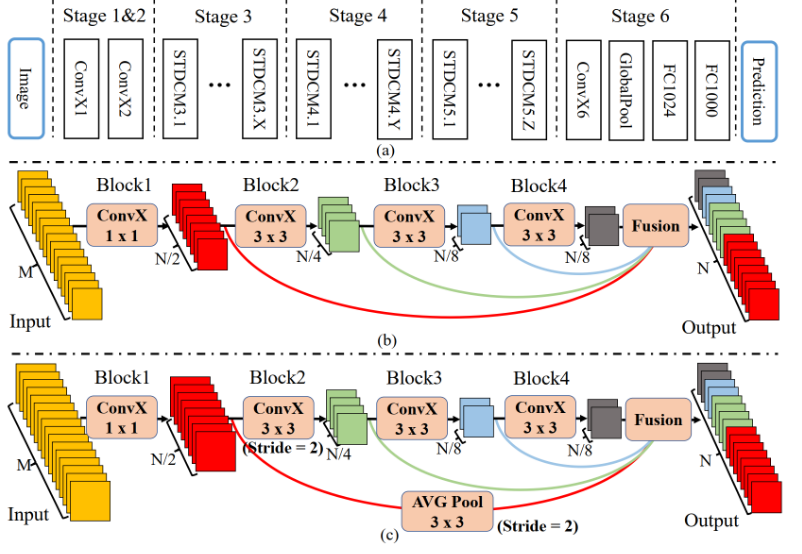
\includegraphics[width=0.4\textwidth]{figures/Figure1-STDCnet.png}}
\caption{STDC network.}
\label{stdc_net}
\end{figure}

\section{Related Word}

Chiedere cosa mettere
\section{Methods}

We first introduce the Short-Term Dense Concatenate network (STDC network) and how we used it with BiSeNet \cite{b2},
then the unsupervised adversarial domain adaptation method.

STDC network \cite{b1} is represented in Fig.~\ref{stdc_net} (a). Stage 3,4 and 5 have a number of Short-Term Dense Concatenate Module (STDCM)
where each module is composed of ConvX blocks Fig.~\ref{stdc_net} (b)(c). Each \(ConvX_i\) is a block composed of one convolutional layer,
one batch normalization layer and one ReLU activation layer. The ConvX layers filter the input into N/2, where N is the channel number
of the STDC module. At the end we concatenate the output of each ConvX block as follow: 
\[x_{output} = F(x_1,x_2,...,x_n)\]
where \(x_{output}\) is the STDC module output, \(F\) is the fusion operation, that in our case is the concatenation and \(x_1,x_2,
...,x_n\) are the output of each \(ConvX_i\) block.

This STDC network is then used as backbone for the context path of BiSeNet, in particular we use stage 3,4 and 5 to reduce the 
feature map to obtain large receptive field. Then a global avarage pooling in added on the tial of the context path. We also use
Attention Refine Module (ARM) on Stage 4 and 5. Finally a Future Fusion Model (FFM) is used to fuse the 1/8
feature from Stage 3 with this last part.

The main idea of the unsupervised adversarial domain adaptation method \cite{b3} is to create a segmentation network that classify the source
image (that as a label) and the target image (without annotations). Then those two predictions are given to the discriminator that
has to distinguish whether the input is from source or target domain. To do so we need a loss from the discriminator to the 
segmentation network which encourage the segmentation to generate similar preditions. We use as segmentation newtork the BiSeNet 
developed above. The loss is 
\[L(I_s,I_t) = L_{seg}(I_s) + \lambda_{adv}*L_{adv}(I_t)\]
where \(L_{seg}\) is the cross entropy loss for the prediction of the source domain, \(\lambda_{adv}\) is the weight used to 
balance the \(L_{adv}\) that is a BCEWithLogitLoss.
We first forward \(I_s\) to the segmentation newtork to get the predition \(P_s\) and the loss \(L_{seg}\). Then forward \(I_t\) to
the segmentation network to get the predition \(P_t\) and feed these two predition to the discriminator.
CHIEDERE DISCRIMINATORE a cosa serve la lossd

\section{Experiments}

We have done the following experiments: (1) train on Cityscapes and test on Cityscapes, (2) train on GTA5 and test on GTA5, (3) train on 
GTA5 and test on Cityscapes without domain adaptation, (4) train on GTA5 and test on Cityscapes without domain adaptation with some
augmentation on GTA5, (5) train on GTA5 and test on Cityscapes with domain adaptation and (6) train on GTA5 and test on Cityscapes with
domain adaptation with a lighter discriminator. 
We use as optimizer the SGD (Stocastic Gradient Descent) with momentum set at 0.9 and weight decay at \(5e^{-4}\). We use a batch size of 
2 and poly learning rate where the learning rate is updated as follow \(lr = init\_lr * (1 - \frac{iter}{max\_iter})^{power}\), where
\(init\_lr\) is 0.01, \(iter\) is the actual epoch, \(max\_iter\) is the number of epochs and \(power\) is 0.9. Data augmentation, when
used, contains Color Jitter, Random Horizontal Flip, Random Crop and Normalization. The disciminator for the domain apadtation part
is trained using Adam with a poly learning rate with the same parameter as before. 
We perform our experiments with those versions:\textbf{TODO!!!!!!!!!}

(1) Here we trained our model on Cityscapes train set and test it on Cityscapes validation set. Here there's no domain adaptation, so
we expect to have high results. Table~\ref{CityscapesToCityscapes} shows the results.

(2) We train our model on GTA5 train set and test it on GTA5 validation set. Again we expect high results.  
Table~\ref{GTATOGTA} shows the results.

(3) Here we evaluate the domain shift between GTA5 and Cityscapes. We train on GTA5 train set and test on Cityscapes validation set.
Here we don't have any domain adaptation method, so we expect bad results. Table~\ref{GTATOCITYSCAPESNOADAP} shows the results. We can 
see that the mIoU is low, this because the source domain and target domain are different. 

(4) Again we evaluate the domain shift between GTA5 and Cityscapes, but this time with some augmentation on GTA5. Table~\ref{GTATOCITYSCAPESNOADAPAUG}
shows the results and again the mIoU is low beacause of the domain shift.

(5) Here we have domain adaptation \cite{b3}. So we train on GTA5 and test on Cityscapes, but this time we train also the discriminator
with the segmentation network. Table~\ref{GTATOCITYSCAPESADAP} shows the results. We can see a slight improvement of performance
in the mIoU of 3\% with respect to (4).

(6) Finally we implement depthwise convolution in the discriminator. Again same thing as (5) but with a lighter discriminator. Table
~\ref{GTATOCITYSCAPESADAPLIGHT} shows the results. 



\begin{table}[tb]
\caption{Train on Cityscapes train set and test it Cityscapes val set}
\begin{center}
\begin{tabular}{|c|c|c|}
\hline
\multicolumn{3}{|c|}{\textbf{Cityscapes -$>$ Cityscapes}} \\
\cline{1-3} 
\textbf{\textit{Accuracy (\%)}}& \textbf{\textit{mIoU (\%)}}& \textbf{\textit{Train time (avg per-epoch)}} \\
\hline
81.1& 58.6& 2.5 minutes   \\
\hline
\end{tabular}
\label{CityscapesToCityscapes}
\end{center}
\end{table}

\begin{table}[tb]
\caption{Train on GTA5 train set and test it GTA5 val set}
\begin{center}
\begin{tabular}{|c|c|c|}
\hline
\multicolumn{3}{|c|}{\textbf{GTA5 -$>$ GTA5}} \\
\cline{1-3} 
\textbf{\textit{Accuracy (\%)}}& \textbf{\textit{mIoU (\%)}}& \textbf{\textit{Train time (avg per-epoch)}} \\
\hline
80.82& 62.36& 3,4 minutes   \\
\hline
\end{tabular}
\label{GTATOGTA}
\end{center}
\end{table}

\begin{table}[tb]
\caption{Train on GTA5 train set and test it Cityscapes val set without adaptation}
\begin{center}
\begin{tabular}{|c|c|c|}
\hline
\multicolumn{3}{|c|}{\textbf{GTA5 -$>$ Cityscapes}} \\
\cline{1-3} 
\textbf{\textit{Accuracy (\%)}}& \textbf{\textit{mIoU (\%)}}& \textbf{\textit{Train time (avg per-epoch)}} \\
\hline
& & \\
\hline
\end{tabular}
\label{GTATOCITYSCAPESNOADAP}
\end{center}
\end{table}

\begin{table}[tb]
\caption{Train on GTA5 augemnted train set and test it Cityscapes val set without adaptation}
\begin{center}
\begin{tabular}{|c|c|c|}
\hline
\multicolumn{3}{|c|}{\textbf{GTA5 -$>$ Cityscapes}} \\
\cline{1-3} 
\textbf{\textit{Accuracy (\%)}}& \textbf{\textit{mIoU (\%)}}& \textbf{\textit{Train time (avg per-epoch)}} \\
\hline
71 & 30 & 5.37 minutes \\
\hline
\end{tabular}
\label{GTATOCITYSCAPESNOADAPAUG}
\end{center}
\end{table}

\begin{table}[tb]
\caption{Train on GTA5 augemnted train set and test it Cityscapes val set with adaptation}
\begin{center}
\begin{tabular}{|c|c|c|}
\hline
\multicolumn{3}{|c|}{\textbf{GTA5 -$>$ Cityscapes}} \\
\cline{1-3} 
\textbf{\textit{Accuracy (\%)}}& \textbf{\textit{mIoU (\%)}}& \textbf{\textit{Train time (avg per-epoch)}} \\
\hline
74 & 33 & 4.55 minutes \\
\hline
\end{tabular}
\label{GTATOCITYSCAPESADAP}
\end{center}
\end{table}

\begin{table}[tb]
\caption{Train on GTA5 augemnted train set and test it Cityscapes val set with lighter adaptation}
\begin{center}
\begin{tabular}{|c|c|c|}
\hline
\multicolumn{3}{|c|}{\textbf{GTA5 -$>$ Cityscapes}} \\
\cline{1-3} 
\textbf{\textit{Accuracy (\%)}}& \textbf{\textit{mIoU (\%)}}& \textbf{\textit{Train time (avg per-epoch)}} \\
\hline
73& 32.5& 4.5 minutes\\
\hline
\end{tabular}
\label{GTATOCITYSCAPESADAPLIGHT}
\end{center}
\end{table}

\section{Conclusion}

\section{Ease of Use}

\subsection{Maintaining the Integrity of the Specifications}

The IEEEtran class file is used to format your paper and style the text. All margins, 
column widths, line spaces, and text fonts are prescribed; please do not 
alter them. You may note peculiarities. For example, the head margin
measures proportionately more than is customary. This measurement 
and others are deliberate, using specifications that anticipate your paper 
as one part of the entire proceedings, and not as an independent document. 
Please do not revise any of the current designations.

\section{Prepare Your Paper Before Styling}
Before you begin to format your paper, first write and save the content as a 
separate text file. Complete all content and organizational editing before 
formatting. Please note sections \ref{AA}--\ref{SCM} below for more information on 
proofreading, spelling and grammar.

Keep your text and graphic files separate until after the text has been 
formatted and styled. Do not number text heads---{\LaTeX} will do that 
for you.

\subsection{Abbreviations and Acronyms}\label{AA}
Define abbreviations and acronyms the first time they are used in the text, 
even after they have been defined in the abstract. Abbreviations such as 
IEEE, SI, MKS, CGS, ac, dc, and rms do not have to be defined. Do not use 
abbreviations in the title or heads unless they are unavoidable.

\subsection{Units}
\begin{itemize}
\item Use either SI (MKS) or CGS as primary units. (SI units are encouraged.) English units may be used as secondary units (in parentheses). An exception would be the use of English units as identifiers in trade, such as ``3.5-inch disk drive''.
\item Avoid combining SI and CGS units, such as current in amperes and magnetic field in oersteds. This often leads to confusion because equations do not balance dimensionally. If you must use mixed units, clearly state the units for each quantity that you use in an equation.
\item Do not mix complete spellings and abbreviations of units: ``Wb/m\textsuperscript{2}'' or ``webers per square meter'', not ``webers/m\textsuperscript{2}''. Spell out units when they appear in text: ``. . . a few henries'', not ``. . . a few H''.
\item Use a zero before decimal points: ``0.25'', not ``.25''. Use ``cm\textsuperscript{3}'', not ``cc''.)
\end{itemize}

\subsection{Equations}
Number equations consecutively. To make your 
equations more compact, you may use the solidus (~/~), the exp function, or 
appropriate exponents. Italicize Roman symbols for quantities and variables, 
but not Greek symbols. Use a long dash rather than a hyphen for a minus 
sign. Punctuate equations with commas or periods when they are part of a 
sentence, as in:
\begin{equation}
a+b=\gamma\label{eq}
\end{equation}

Be sure that the 
symbols in your equation have been defined before or immediately following 
the equation. Use ``\eqref{eq}'', not ``Eq.~\eqref{eq}'' or ``equation \eqref{eq}'', except at 
the beginning of a sentence: ``Equation \eqref{eq} is . . .''

\subsection{\LaTeX-Specific Advice}

Please use ``soft'' (e.g., \verb|\eqref{Eq}|) cross references instead
of ``hard'' references (e.g., \verb|(1)|). That will make it possible
to combine sections, add equations, or change the order of figures or
citations without having to go through the file line by line.

Please don't use the \verb|{eqnarray}| equation environment. Use
\verb|{align}| or \verb|{IEEEeqnarray}| instead. The \verb|{eqnarray}|
environment leaves unsightly spaces around relation symbols.

Please note that the \verb|{subequations}| environment in {\LaTeX}
will increment the main equation counter even when there are no
equation numbers displayed. If you forget that, you might write an
article in which the equation numbers skip from (17) to (20), causing
the copy editors to wonder if you've discovered a new method of
counting.

{\BibTeX} does not work by magic. It doesn't get the bibliographic
data from thin air but from .bib files. If you use {\BibTeX} to produce a
bibliography you must send the .bib files. 

{\LaTeX} can't read your mind. If you assign the same label to a
subsubsection and a table, you might find that Table I has been cross
referenced as Table IV-B3. 

{\LaTeX} does not have precognitive abilities. If you put a
\verb|\label| command before the command that updates the counter it's
supposed to be using, the label will pick up the last counter to be
cross referenced instead. In particular, a \verb|\label| command
should not go before the caption of a figure or a table.

Do not use \verb|\nonumber| inside the \verb|{array}| environment. It
will not stop equation numbers inside \verb|{array}| (there won't be
any anyway) and it might stop a wanted equation number in the
surrounding equation.

\subsection{Some Common Mistakes}\label{SCM}
\begin{itemize}
\item The word ``data'' is plural, not singular.
\item The subscript for the permeability of vacuum $\mu_{0}$, and other common scientific constants, is zero with subscript formatting, not a lowercase letter ``o''.
\item In American English, commas, semicolons, periods, question and exclamation marks are located within quotation marks only when a complete thought or name is cited, such as a title or full quotation. When quotation marks are used, instead of a bold or italic typeface, to highlight a word or phrase, punctuation should appear outside of the quotation marks. A parenthetical phrase or statement at the end of a sentence is punctuated outside of the closing parenthesis (like this). (A parenthetical sentence is punctuated within the parentheses.)
\item A graph within a graph is an ``inset'', not an ``insert''. The word alternatively is preferred to the word ``alternately'' (unless you really mean something that alternates).
\item Do not use the word ``essentially'' to mean ``approximately'' or ``effectively''.
\item In your paper title, if the words ``that uses'' can accurately replace the word ``using'', capitalize the ``u''; if not, keep using lower-cased.
\item Be aware of the different meanings of the homophones ``affect'' and ``effect'', ``complement'' and ``compliment'', ``discreet'' and ``discrete'', ``principal'' and ``principle''.
\item Do not confuse ``imply'' and ``infer''.
\item The prefix ``non'' is not a word; it should be joined to the word it modifies, usually without a hyphen.
\item There is no period after the ``et'' in the Latin abbreviation ``et al.''.
\item The abbreviation ``i.e.'' means ``that is'', and the abbreviation ``e.g.'' means ``for example''.
\end{itemize}
An excellent style manual for science writers is \cite{b7}.

\subsection{Authors and Affiliations}
\textbf{The class file is designed for, but not limited to, six authors.} A 
minimum of one author is required for all conference articles. Author names 
should be listed starting from left to right and then moving down to the 
next line. This is the author sequence that will be used in future citations 
and by indexing services. Names should not be listed in columns nor group by 
affiliation. Please keep your affiliations as succinct as possible (for 
example, do not differentiate among departments of the same organization).

\subsection{Identify the Headings}
Headings, or heads, are organizational devices that guide the reader through 
your paper. There are two types: component heads and text heads.

Component heads identify the different components of your paper and are not 
topically subordinate to each other. Examples include Acknowledgments and 
References and, for these, the correct style to use is ``Heading 5''. Use 
``figure caption'' for your Figure captions, and ``table head'' for your 
table title. Run-in heads, such as ``Abstract'', will require you to apply a 
style (in this case, italic) in addition to the style provided by the drop 
down menu to differentiate the head from the text.

Text heads organize the topics on a relational, hierarchical basis. For 
example, the paper title is the primary text head because all subsequent 
material relates and elaborates on this one topic. If there are two or more 
sub-topics, the next level head (uppercase Roman numerals) should be used 
and, conversely, if there are not at least two sub-topics, then no subheads 
should be introduced.

\subsection{Figures and Tables}
\paragraph{Positioning Figures and Tables} Place figures and tables at the top and 
bottom of columns. Avoid placing them in the middle of columns. Large 
figures and tables may span across both columns. Figure captions should be 
below the figures; table heads should appear above the tables. Insert 
figures and tables after they are cited in the text. Use the abbreviation 
``Fig.~\ref{fig}'', even at the beginning of a sentence.

\begin{table}[htbp]
\caption{Table Type Styles}
\begin{center}
\begin{tabular}{|c|c|c|c|}
\hline
\textbf{Table}&\multicolumn{3}{|c|}{\textbf{Table Column Head}} \\
\cline{2-4} 
\textbf{Head} & \textbf{\textit{Table column subhead}}& \textbf{\textit{Subhead}}& \textbf{\textit{Subhead}} \\
\hline
copy& More table copy$^{\mathrm{a}}$& &  \\
\hline
\multicolumn{4}{l}{$^{\mathrm{a}}$Sample of a Table footnote.}
\end{tabular}
\label{tab1}
\end{center}
\end{table}

\begin{figure}[htbp]
\centerline{
\includegraphics{figures/fig1.png}}
\caption{Example of a figure caption.}
\label{fig}
\end{figure}

Figure Labels: Use 8 point Times New Roman for Figure labels. Use words 
rather than symbols or abbreviations when writing Figure axis labels to 
avoid confusing the reader. As an example, write the quantity 
``Magnetization'', or ``Magnetization, M'', not just ``M''. If including 
units in the label, present them within parentheses. Do not label axes only 
with units. In the example, write ``Magnetization (A/m)'' or ``Magnetization 
\{A[m(1)]\}'', not just ``A/m''. Do not label axes with a ratio of 
quantities and units. For example, write ``Temperature (K)'', not 
``Temperature/K''.

\section*{Acknowledgment}

The preferred spelling of the word ``acknowledgment'' in America is without 
an ``e'' after the ``g''. Avoid the stilted expression ``one of us (R. B. 
G.) thanks $\ldots$''. Instead, try ``R. B. G. thanks$\ldots$''. Put sponsor 
acknowledgments in the unnumbered footnote on the first page.

\section*{References}

Please number citations consecutively within brackets \cite{b1}. The 
sentence punctuation follows the bracket \cite{b2}. Refer simply to the reference 
number, as in \cite{b3}---do not use ``Ref. \cite{b3}'' or ``reference \cite{b3}'' except at 
the beginning of a sentence: ``Reference \cite{b3} was the first $\ldots$''

Number footnotes separately in superscripts. Place the actual footnote at 
the bottom of the column in which it was cited. Do not put footnotes in the 
abstract or reference list. Use letters for table footnotes.

Unless there are six authors or more give all authors' names; do not use 
``et al.''. Papers that have not been published, even if they have been 
submitted for publication, should be cited as ``unpublished'' \cite{b4}. Papers 
that have been accepted for publication should be cited as ``in press'' \cite{b5}. 
Capitalize only the first word in a paper title, except for proper nouns and 
element symbols.

For papers published in translation journals, please give the English 
citation first, followed by the original foreign-language citation \cite{b6}.

\begin{thebibliography}{00}
\bibitem{b1} G. Eason, B. Noble, and I. N. Sneddon, ``On certain integrals of Lipschitz-Hankel type involving products of Bessel functions,'' Phil. Trans. Roy. Soc. London, vol. A247, pp. 529--551, April 1955.
\bibitem{b2} J. Clerk Maxwell, A Treatise on Electricity and Magnetism, 3rd ed., vol. 2. Oxford: Clarendon, 1892, pp.68--73.
\bibitem{b3} I. S. Jacobs and C. P. Bean, ``Fine particles, thin films and exchange anisotropy,'' in Magnetism, vol. III, G. T. Rado and H. Suhl, Eds. New York: Academic, 1963, pp. 271--350.
\bibitem{b4} K. Elissa, ``Title of paper if known,'' unpublished.
\bibitem{b5} R. Nicole, ``Title of paper with only first word capitalized,'' J. Name Stand. Abbrev., in press.
\bibitem{b6} Y. Yorozu, M. Hirano, K. Oka, and Y. Tagawa, ``Electron spectroscopy studies on magneto-optical media and plastic substrate interface,'' IEEE Transl. J. Magn. Japan, vol. 2, pp. 740--741, August 1987 [Digests 9th Annual Conf. Magnetics Japan, p. 301, 1982].
\bibitem{b7} M. Young, The Technical Writer's Handbook. Mill Valley, CA: University Science, 1989.
\end{thebibliography}
\vspace{12pt}
\color{red}
IEEE conference templates contain guidance text for composing and formatting conference papers. Please ensure that all template text is removed from your conference paper prior to submission to the conference. Failure to remove the template text from your paper may result in your paper not being published.

\end{document}
